
\documentclass{article}
\usepackage{graphicx}

\begin{document}
\title{Spécifiation des exigences du modèle : Jalon 1}

\author{Louis-Vincent CAPELLI \and Alexandre THEISSE \and Tom SARTORI \and Raphaël TURCOTTE}
\date{\today}
\maketitle
\newpage

\tableofcontents
\newpage

\section{Introduction}
\subsection*{Objet et portée du document}
Ce document a pour but de spécifier les exigences du jalon 1 du projet "Système
de surveillance de la qualité de l'air" (SSQA). Il est destiné aux membres du 
groupe de travail, afin de leur permettre de cerner correctement les besoins
du client et de les retranscrire lors de la conception.

\section{Présentation}
\subsection{Mise en contexte}
Une première analyse a conduit à l'élaboration du schéma préliminaire présenté ci-après.
Il prend la forme d'un diagramme relationnel.

\begin{figure}[h]
\centering
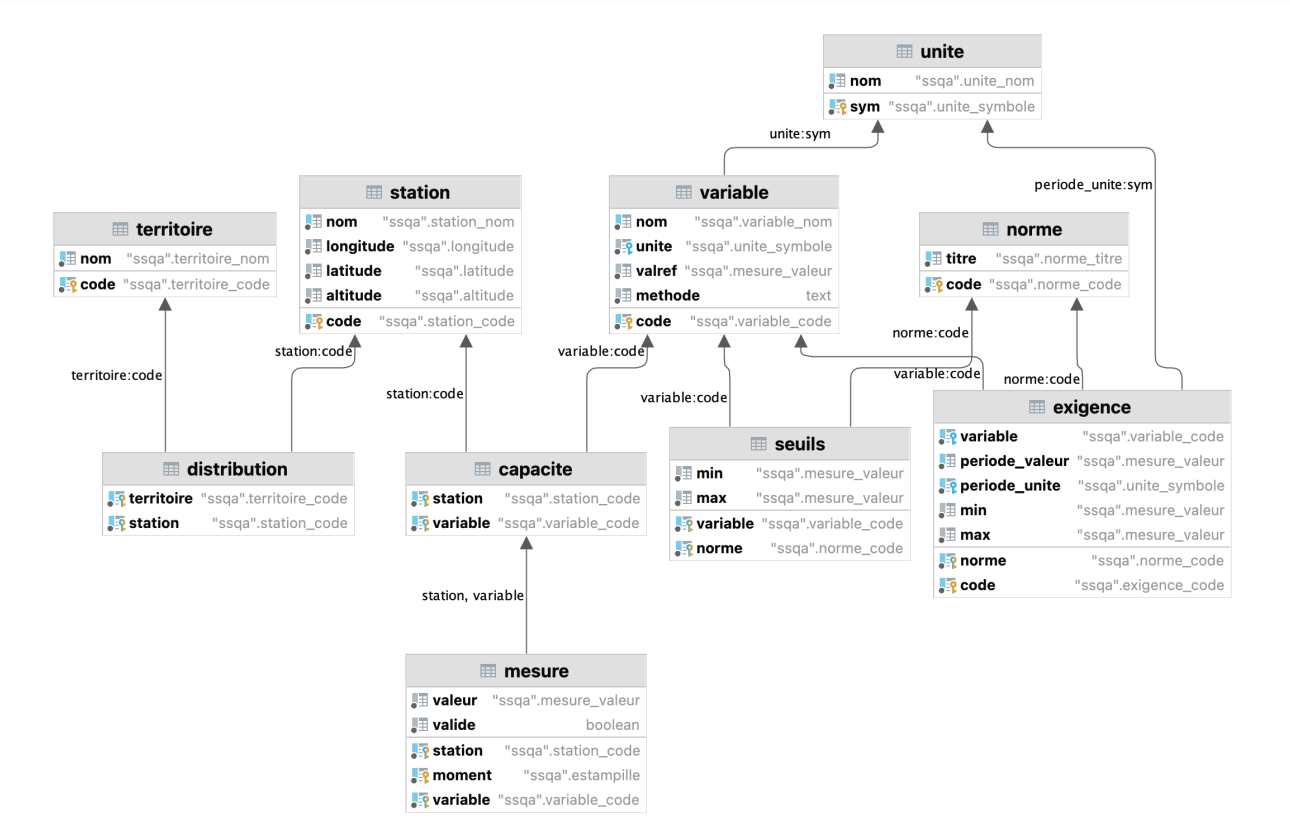
\includegraphics[scale=0.4]{preli.png}
\caption{Schéma préliminaire}
\end{figure}

\subsection{Système existant}
Le système existant est une base de données PostgreSQL correspondante
au schéma préliminaire ci-dessus. Les scripts de création de la base de données ont
été fournis par le client.

\section{Problème}
Ce jalon porte principalement sur la modification du schéma préliminaire, afin
de le rendre plus conforme à une utilisation en situation réelle. Il s'agit donc de
faire évoluer la base de données SSQA en cours d'exploitation afin de couvrir
les besoins du client. Ces modifications portent principalement sur la représentation
des unités dans la base de données et sur la manière de gérer la validité des 
mesures effectuées par les différentes stations.

\section{Exigences}
\subsection{Exigences fonctionnelles}
\subsubsection{R01.SI\_mod}
\paragraph{Description} Représenter toutes les unités en fonction des unités fondamentales définies par le SI
et de deux coefficients additif et multiplicatif.

\paragraph{Prolongements possibles}
\begin{itemize}
    \item Permettre la définition d'unités fondamentales supplémentaires (par exemple, le bit).
    \item Fournir une fonction de représentation des mesures utilisant optimalement les préfixes du SI (par exemple, 1.2 kbit).
\end{itemize}


\subsubsection{R02.SI\_sym}
\paragraph{Description} Restreindre les symboles des unités grace aux règles du BIPM.


\subsubsection{R04.Variable\_contrainte}
\paragraph{Description} 
\begin{itemize}
    \item Vérifier que la valeur de référence de la variable est comprise dans l'intervalle de
    validité fixé par la norme associée.
    \item Vérifier que les min et max des exigences pour une variable sont compris
    dans l'intervalle de validité fixé par la norme associée pour cette variable.
\end{itemize}


\subsubsection{R06.Station\_service}
\paragraph{Description} Afin de permettre de valider les temps des mesures :
ajouter les attributs de mise en exploitation et de fin d'exploitation de la station et 
maintenir une table des périodes d'entretien ou de non-disponibilité des stations.


\subsubsection{R07.Station\_mobilité}
\paragraph{Description} Certaines stations sont mobiles, leurs coordonnées varient donc dans le temps. Les stations fixes peuvent aussi
être déplacées à l'occasion. Ainsi il faudra modifier le schéma afin 
de pouvoir consigner l'évolution des coordonnées des stations.


\subsubsection{R08.Validation\_période}
\paragraph{Description} Vérifier que l'attribut periode\_unite de la table Exigence
est une unité de temps valide.


\subsubsection{R09.Station\_nom\_facultatif}
\paragraph{Description} Une station n'a pas forcément de nom, son emplacement
est alors utilisé pour la désigner. Rendre le nom de la station facultatif 
dans la mesure ou elle n'est pas mobile.


\subsubsection{R10.Mesure\_valeur\_absente}
\paragraph{Description} Rendre la valeur d'une mesure facultative, et modifier la base de données
afin de pouvoir conserver la cause de l'absence de mesure.


\subsection{Exigences non-fonctionnelles}
\subsubsection{R03.Validation\_nom}
\paragraph{Description} Changer le nom de la table "Seuils" pour "Validation"
et faire percoler les conséquences de ce changement dans le reste de la base de données.


\subsubsection{R05.Méthode\_codification}
\paragraph{Description} Les méthodes d'échantillonnage des variables sont en texte libre, ce qui laisse place à des erreurs de saisie qui
pourraient résulter en la définition de plusieurs représentations pour une même méthode. Afin de mieux valider les données, les méthodes devraient être codifiées.


\subsubsection{R11.Documentation}
\paragraph{Description} Afin d'assurer l'interprétation correcte des données, associer
le texte complet de chaque prédicat ainsi que ses dépendances fonctionnelles à l'aide
d'un commentaire inscrit au catalogue.

\end{document}
